% Chapter 5

\chapter{Instrumentation Performance} % Write in your own chapter title
\label{Chapter5}
\lhead{Chapter 5. \emph{Performance}} % Write in your own chapter title to set the page header

\section{SFC}

\subsection{Restrictor blockage}

Figure~\ref{fig:RestrictorEnd} is a SEM image of the end of the restrictor used to depressurize the supercritical carbon dioxide. 

\begin{figure}[htbp]
	\centering
	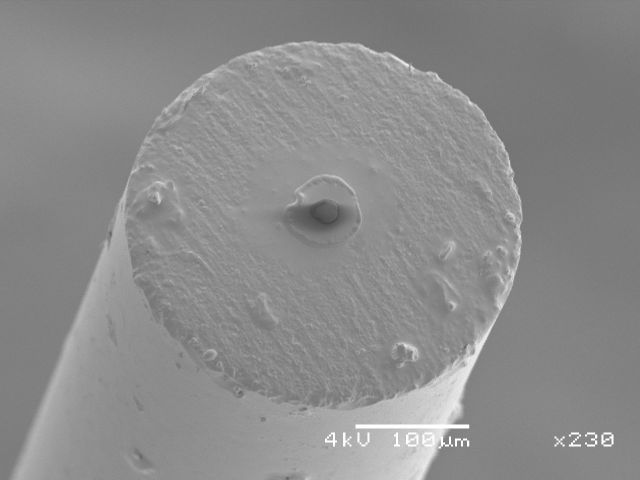
\includegraphics[width=0.8\textwidth,natwidth=4.17in,natheight=3.32in]{./Figures/RestrictorEnd.jpg}
	\rule{35em}{0.5pt}
	\caption[A SEM image of a restrictor orifice]{A SEM image of a restrictor orifice. The grinding marks of the 2000 grit grinding medium can be clearly seen on the end of the capillary. The left-to-right dark `smudge' around the orifice is cause by some charging of the hole in the electorn microscope, because the gold sputtering process does not coat the inside of holes very easily.}
	\label{fig:RestrictorEnd}
\end{figure}

From time to time this restrictor got plugged. Initially it was though that this plugging was caused by particles from the valve system and the columns, and the plugging . The size of the hole was not known, because the end of the restrictor was ground down until the hole was the right size for the desired flow. What was known was that the hole was too small to be visible to the naked eye or under a low-power stereo microscope. A higher-powered stereo microscope at the Unit for Microscopy and Microanalysis at the University of Pretoria showed that the hole is about 10 to 20 micron in diameter, which answered one question: since the 0.5$\mu$m filter should remove all the smaller particles, a 20 $\mu$m orifice will easily pass any particles let through by the filter. Even the 3 $\mu$m column packing particles will not plug this hole. Therefore it seems very unlikely that single particles cause the plugging.

The possibility exists that an excess of small particles may clot and form a plug. 

Taking the SEM image confirmed the size of the hole, but revealed something else. This particular restrictor had plugged, but had been ground again to recover flow. Around the hole there is visible an `island' of different texture. A SEM image in backscatter mode (Figure~\ref{fig:RestrictorHole}) shows that the chemistry of this `island' is different from the chemistry of the surrounding silica. The morphology also suggests that it is a much softer material, it not exhibiting grinding marks and appearing to have flowed.

\begin{figure}[htbp]
	\centering
	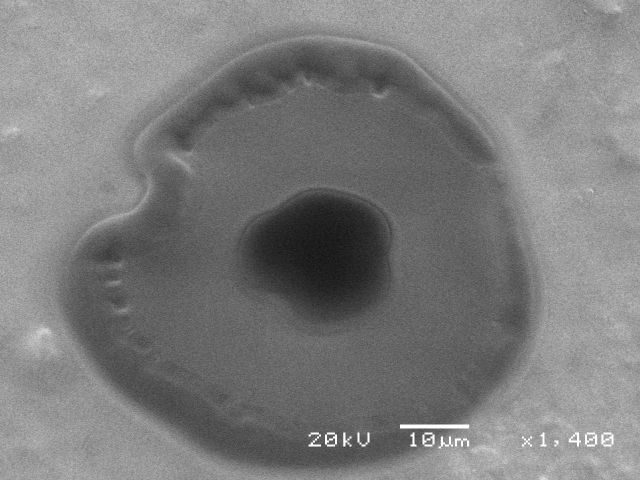
\includegraphics[width=0.8\textwidth,natwidth=4.17in,natheight=3.32in]{./Figures/RestrictorHole.jpg}
	\rule{35em}{0.5pt}
	\caption[Restrictor Ofrifice]{The end of restrictor, showing the size of the orifice.}
	\label{fig:RestrictorHole}
\end{figure}

What is clear is that there is no evidence of particulate matter plugging the orifice.

There is a possibility that this softer material is the actual blocking matter. There are some proposed origins for this material.
\begin{itemize}
	\item It might be polymeric material formed in the sample that got transported through the system and precipitated in the restrictor. (We have found polymeric material in essential oils.)
	\item It might be sample material that separated in the SFC column, but precipitated during the SFC cycling on and off, and failed to re-dissolve during subsequent cycles because conditions different from the injection and separation parts of the SFC made dissolution kinetically unfavourable.
	\item It might be sample material that precipitated during the pressure cycles of the SFC going into stopped-flow, and then polymerised or carbonised in the hot inlet.
	\item It might be that the capillary is not manufactured of uniform material but contains a softer core around the lumen of the capillary.
\end{itemize}

\section{Fast GC}

\section{Heating and cooling rates}

In previous work using SFC�GC, the metal column was cooled by using the cryogenic cooling function of the Varian 3300 oven. This function works by injection liquid carbon dioxide into the oven, behind the air circulating fan. This ensures a cooling of the whole oven. But this function of the Varian was intended for the cooling of the oven once for every normal GC run, which would mean cooling at most every 10 minutes or so. Using the fast GC column to trap small fractions of SFC eluent means the very frequent cooling of the whole oven. Although the oven is not deliberately heated, heat from the heated inlet and detector would still leak into the oven.

These workers reported [Makgwane2006] that the system used a lot of carbon dioxide for cooling.

When we started using the coaxial capillary heater, we welded wires to the stainless steel heater capillary. To prevent creating cold spots on the column, we added heater blocks to the junctions, close to the inlet and detector, to ensure an evenly heated area where the conductor joins the coaxial heater. Though it was thermally isolated, more heat still leaked into the oven. 

In our experience, the total cooling required for this system was about half a bottle (approximately 16 kg) of technical grade carbon dioxide per 2D chromatographic run. 

This is an unacceptably high consumption of carbon dioxide, both in terms of cost and of unnecessary carbon emission. That costs about ZAR 3.56 just in carbon costs per run. 

% On the 1st of July 2012 the Australian Federal government introduced a carbon price, a price of $23AUD per tonne of emitted CO2-e on selected fossil fuels consumed by major industrial emitters only.
% That's ZAR 216 per tonne. 21.6 per kilogram. 

So it was decided to take the step to cool the column only, using the concept of the capillary coaxial heater, and then blowing the liquid carbon dioxide into the void between the heater and the column. 

The flow needed for this about one tenth of the flow used by the Varian's cryogenic cooling, and the duration of the flow is much less, resulting in a lesser use of carbon dioxide for cooling. 

%Figure showing flow compared between Varian and coaxial cooling. 
\begin{figure}[htbp]
	\centering
%	\includegraphics[width=0.8\textwidth,natwidth=4.17in,natheight=3.32in]{./Figures/filename.pdf}
	\rule{35em}{0.5pt}
	\caption["short"]{"long"}
	\label{fig:TheFigureLabel}
\end{figure}

% Add calculation to show 

The saving in carbon dioxide is significant, but the effort saved in not needing to worry about the coolant running out saves much more effort and energy. A sample run can easily be ruined by the coolant running out unexpectedly. And as we know, there is no way of determining the contents level of an industrial steel cylinder of liquefied gas. 

\section{Repeatability}

In the work by Venter \cite{Venter2004}\cite{Venter2006} it became apparent that the temperature programme was not too reliable. This was pointed out in a graph that compared the temperature reported by the controlling thermocouple with the temperature reported by a monitoring thermocouple positioned on another part of the metal column. Although the temperature of the controlling thermocouple followed the setpoint of the temperature ramp faithfully, the monitoring thermocouple reported quite a different temperature. The 2D chromatogram of course showed this discrepancy, with the contouring software interpreting the jaggedness of the resulting peaks as separate peaks. 

